% !TeX TXS-program:compile = txs:///pdflatex/[--shell-escape]
\documentclass[10pt,landscape,a4paper]{article}
\usepackage[table]{xcolor}
\usepackage[normalem]{ulem}
\usepackage{tikz}
\usetikzlibrary{shapes,positioning,arrows,fit,calc,graphs,graphs.standard}
\usepackage[nosf]{kpfonts}
\usepackage[t1]{sourcesanspro}
\usepackage{multicol}
\usepackage{wrapfig}
\usepackage[top=1mm,bottom=1mm,left=1mm,right=1mm]{geometry}
\usepackage[framemethod=tikz]{mdframed}
\usepackage{microtype}
\usepackage{tabularx}
\usepackage{hhline}
\usepackage{makecell}
\usepackage{mathtools}
\usepackage{subfig}
\usepackage{listings}
\usepackage{soul}
\usepackage{amsmath,amsthm,amsfonts,amssymb}

\graphicspath{ {./img/} }

\DeclarePairedDelimiter{\ceil}{\lceil}{\rceil}

\definecolor{myblue}{cmyk}{1,.72,0,.38}

\pgfdeclarelayer{background}
\pgfsetlayers{background,main}

\renewcommand{\baselinestretch}{.8}
\pagestyle{empty}

\let\counterwithout\relax
\let\counterwithin\relax
\usepackage{chngcntr}
\usepackage{verbatim}
\usepackage{etoolbox}
\makeatletter
\preto{\@verbatim}{\topsep=0pt \partopsep=0pt }
\makeatother

\counterwithin*{equation}{section}
\counterwithin*{equation}{subsection}
\usepackage{enumitem}
\newlist{legal}{enumerate}{10}
\setlist[legal]{label*=\arabic*.,leftmargin=3mm}
\setlist[itemize]{leftmargin=3mm}
\setlist[enumerate]{leftmargin=3.5mm}
\setlist{nosep}
\usepackage{minted}

\newenvironment{descitemize} % a mixture of description and itemize
{\begin{description}[leftmargin=*,before=\let\makelabel\descitemlabel]}
	{\end{description}}
\newcommand{\descitemlabel}[1]{%
	\textbullet\ \textbf{#1}%
}
\makeatletter

\renewcommand{\section}{\@startsection{section}{1}{0mm}%
	{.2ex}%
	{.2ex}%x
	{\color{myblue}\sffamily\small\bfseries}}
\renewcommand{\subsection}{\@startsection{subsection}{1}{0mm}%
	{.2ex}%
	{.2ex}%x
	{\sffamily\bfseries}}
\renewcommand{\subsubsection}{\@startsection{subsubsection}{1}{0mm}%
	{.2ex}%
	{.2ex}%x
	{\rmfamily\bfseries}}

\makeatother
\setlength{\parindent}{0pt}
\setminted{tabsize=2, breaklines}
% Remove belowskip of minted
\setlength\partopsep{-\topsep}

\newcolumntype{a}{>{\hsize=1.5\hsize}X}
\newcolumntype{b}{>{\hsize=.25\hsize}X}

\setlength\columnsep{10pt}
\setlength\columnseprule{0pt}
\begin{document}
\abovedisplayskip=0pt
\abovedisplayshortskip=0pt
\belowdisplayskip=0pt
\belowdisplayshortskip=0pt
%\scriptsize
\tiny
\begin{multicols*}{4}
\section{Introduction to Computer Security}
\subsection{Possible Attacks}
\begin{enumerate}
	\item Database/Server/Cloud compromise
	\item Insider gains unauthorized access
	\item Network sniffing
	\item Bugs in web app
	\item User impersonation
	\item Password breach
\end{enumerate}
\subsection{Threat Model}
\begin{minipage}{0.2\columnwidth}
	\begin{center}
		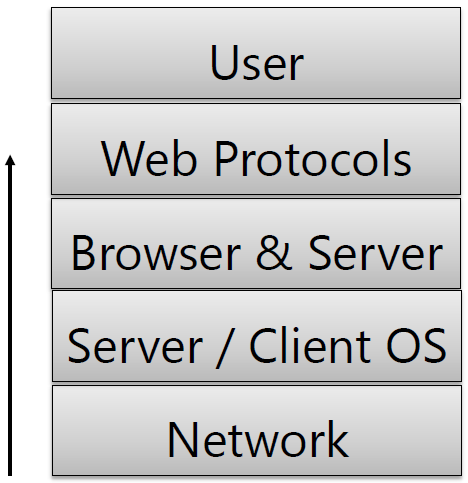
\includegraphics[width=1\columnwidth]{bottom-up}
	\end{center}
\end{minipage}
\begin{minipage}{0.8\columnwidth}
	A threat model defines:
	\begin{itemize}
		\item Desired security property / Goal
		\item Attacker's capability
		\item Assumption about the setup
	\end{itemize}
	Want to argue from a bottom up perspective
\end{minipage}
\subsection{Basic Principles}
\begin{enumerate}
	\item Weakest Link Principal
	\begin{itemize}
		\item Security can be no stronger than its weakest link
		\item e.g. Password can be strong and complicated but "recovering" it requires you to answer simple question
	\end{itemize}
	\item Kerchkhoff’s principal
	\begin{itemize}
		\item Security by Obscurity is bad
	\end{itemize}
\end{enumerate}
\section{Network Attacks}
\subsection{Network Stack}
\begin{center}
	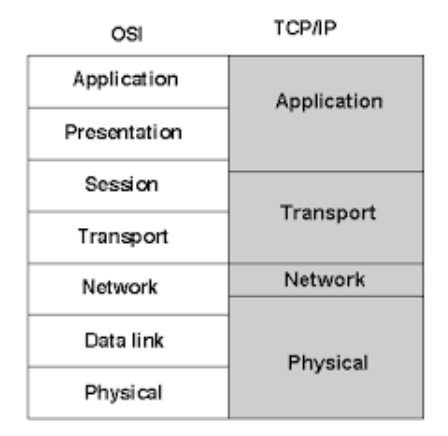
\includegraphics[width=0.3\columnwidth]{network-stack}
\end{center}
\subsection{How the Internet works?}
\begin{minipage}{0.6\columnwidth}
	\begin{center}
		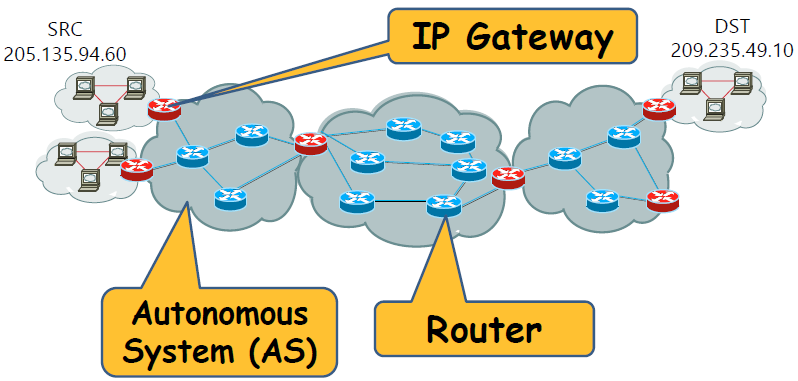
\includegraphics[width=1\columnwidth]{network-diagram}
	\end{center}
\end{minipage}
\begin{minipage}{0.4\columnwidth}
	\begin{itemize}
		\item Built upon a collection of sub-networks
		\item Each of them sitting on an ISP (\textbf{Autonomous System})
		\item ISPs can be thought of as "special routers" that runs on \textbf{BGP}
	\end{itemize}
\end{minipage}
\subsubsection{BGP (TCP/IP: Physical layer)}
\begin{itemize}
	\item Uses NLRI Update (Network Layer Reachability Information) to propagate information
	\item Each ISP broadcast to other ISP the shortest path they know to reach a certain node
\end{itemize}
\begin{center}
	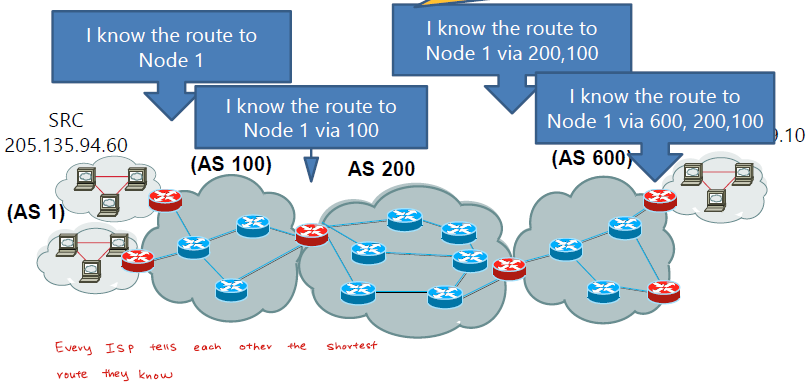
\includegraphics[width=0.6\columnwidth]{bgp}
\end{center}
\subsection{IP Protocol}
IP information is kept in a IP routing table that looks like this:
\begin{tabular}{ c | c | c | c }
	Destination & Gateway & Genmask & Flag \\\hline
	0.0.0.0 & 71.46.14.1 & 0.0.0.0 & UG \\
	10.0.0.0 & 0.0.0.0 & 255.0.0.0 & U \\
	71.46.14.1 & 0.0.0.0 & 255.255.255.255 & UH
\end{tabular}

* Default destination is 0.0.0.0

* Default gateway is the node in a network using the IP protocol that serves as the forwarding host (router) to other networks when no other route matches the destination IP of a packet
\subsection{UDP \& TCP}
\begin{itemize}
	\item Unreliable Data delivery over IP: UDP (packets may or may not be received)
	\item “Reliable” Data Delivery: TCP
	\begin{itemize}
		\item Connection-oriented, ordered packets
	\end{itemize}
\end{itemize}
\subsection{Network Attacks}
\subsubsection{Basic terms}
\begin{itemize}
	\item Eve - passive attacker, can listen to message but cannot modify
	\item Mallory - malicious attacker, aka MITM, can modify messages, substitute messages, or replay old messages
\end{itemize}
\subsubsection{BGP Attacks}
\begin{minipage}{0.5\columnwidth}
	\begin{center}
		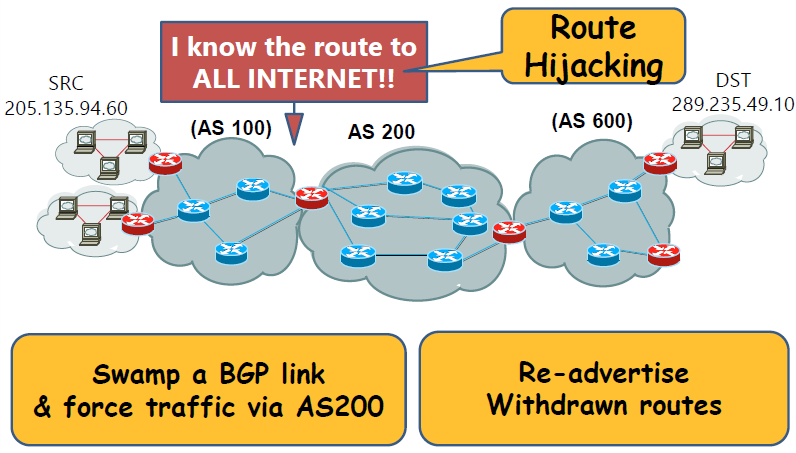
\includegraphics[width=1\columnwidth]{bgp-attack}
	\end{center}
\end{minipage}
\begin{minipage}{0.5\columnwidth}
	\begin{itemize}
		\item Attacker impersonate IP gateway and broadcast that it knows the route to the whole internet
		\item Falsely broadcast that shortest route to all of internet is through a certain ISP to swamp the link
		\item Flaws of BGP:
		\begin{itemize}
			\item Lack of security: no built-in mechanisms for authenticating BGP messages or ensuring the integrity of routing information
			\item Trust-based model: AS trust information sent by other AS
			\item No route validation
		\end{itemize}
	\end{itemize}
\end{minipage}

\subsubsection{IP Attacks}
\begin{minipage}{0.5\columnwidth}
	\begin{center}
		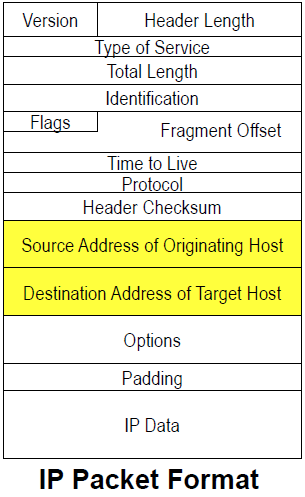
\includegraphics[width=0.4\columnwidth]{ip-packet}
	\end{center}
\end{minipage}
\begin{minipage}{0.5\columnwidth}
	\begin{itemize}
		\item Confidentiality attack: 
		\begin{itemize}
			\item Packet Sniffing
		\end{itemize}
		\item Integrity attack:
		\begin{itemize}
			\item IP data pollution
			\item Source IP forgery - used for DDoS and anonymous infection (e.g. Slammer worm)
		\end{itemize} 
	\end{itemize}
\end{minipage}
\vfill\null\columnbreak
\subsubsection{Slammer Worm}
\begin{itemize}
	\item Swamps UDP port 1434 by generating large amounts of packets
	\item Causes buffer overflow which results in network failure or major slowdown
	\item Uses randomized SRC IP to conceal attacker's IP as well as to bypass firewalls NIDS
\end{itemize}
\subsubsection{Smurf Attacks}
\begin{itemize}
	\item Attacker send a ICMP (ping) packet with DST field being the broadcast IP and DST being the victims IP (DDoS attack)
	\item Also called amplify attack
	\item Takes advantage of other computer in the network to swamp victim with lots of ping requests
	\item Easy to fix now - just block ICMP channel
\end{itemize}
\subsubsection{TCP Attacks}
Sequence Number Prediction
\begin{itemize}
	\item If TCP uses predictable sequence number for their SYN/ACK e.g. always +k, then an attacker can predict the next sequence number and inject message
	\item The other party would still assume that it is talking to the correct person since the numbers match up
	\item Takes advantage of IP authentication which is a weak security protocol
	\item Solution: randomize the sequence number and also increase the number of bits to make it harder for attacker to guess
\end{itemize}
\begin{center}
	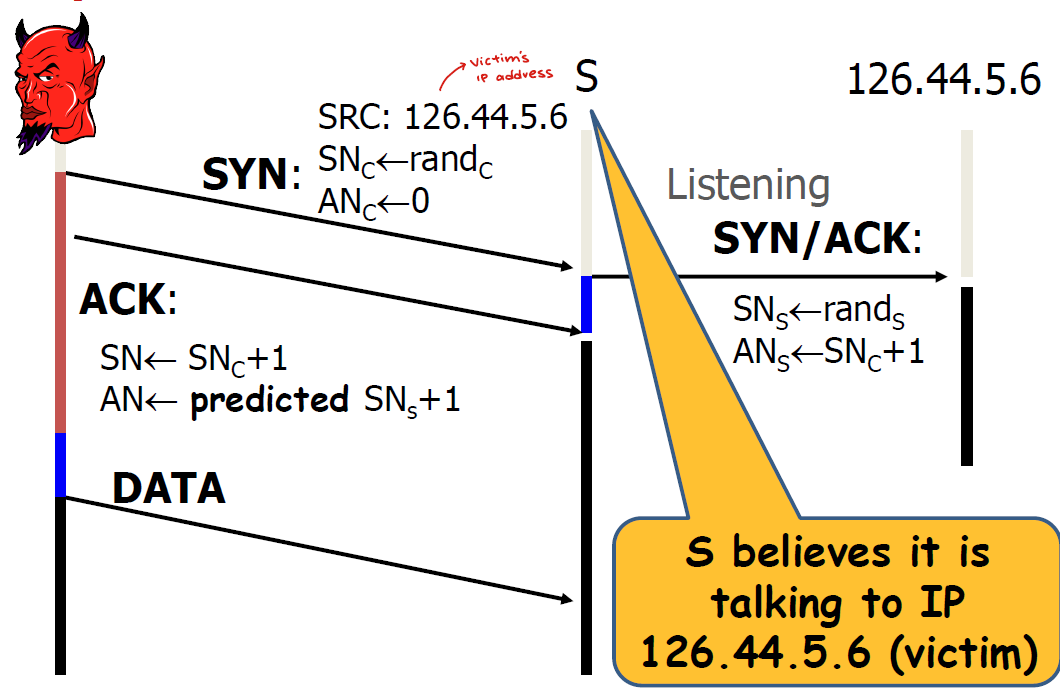
\includegraphics[width=0.55\columnwidth]{tcp-attack}
\end{center}
\subsubsection{DNS Attacks}
\begin{center}
	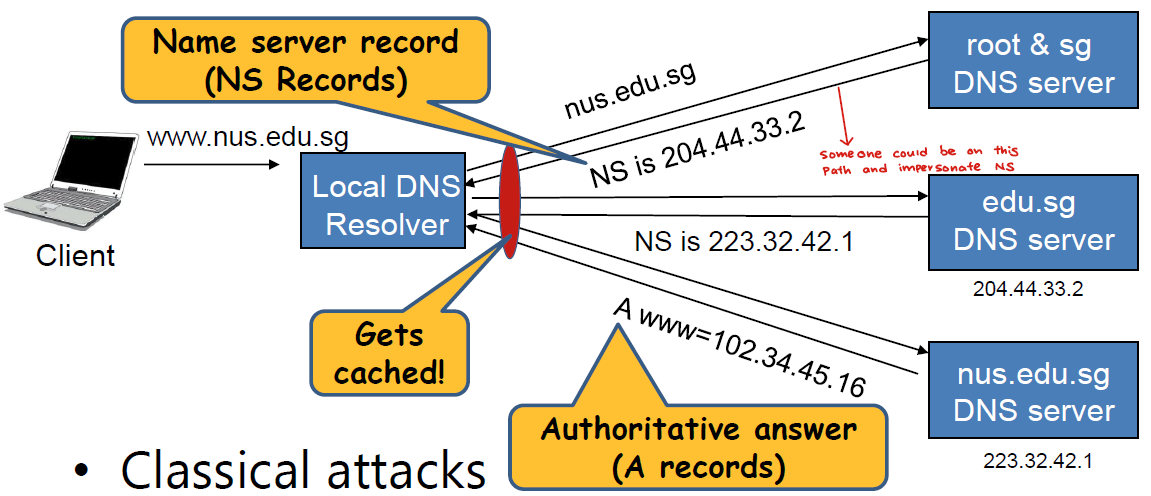
\includegraphics[width=0.7\columnwidth]{dns}
\end{center}
\begin{itemize}
	\item Flaw in DNS resolving is that the QID used is predictable
	\item Possible to carry out DNS Cache poisoning
\end{itemize}
\begin{center}
	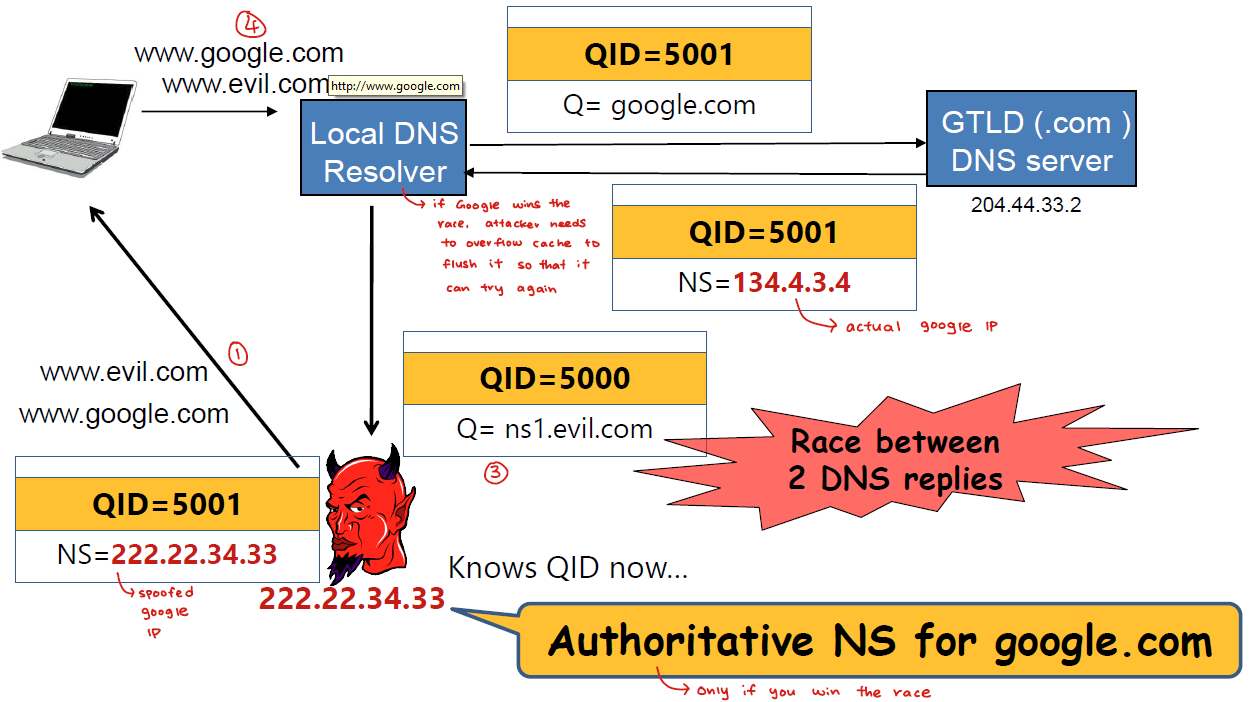
\includegraphics[width=0.7\columnwidth]{dns-poisoning}
\end{center}
\begin{enumerate}
	\item Victim DNS query to resolver for google and some evil website (victim don't even need to click on evil website, could just be an injected JS/img with src of evil website)
	\item DNS tries to resolve for evil.com first
	\item QID will be known to attacker which he then uses to generate a response for Google.com with QID' = QID + 1
	\item If attacker wins the DNS response (could be that the attacker is physically close to the victim) then the DNS will save evil.com NS as Google.com NS
	\item Attacker becomes the authoritative NS for Google.com
\end{enumerate}
\subsection{Firewalls}
Firewalls are tools that control the flow of traffic going between networks.
\begin{itemize}
	\item Sits at border between networks
	\item Looks at services, addresses, data etc. of traffic
	\item Decides whether a packet should be allowed or dropped based on a firewall policy
	\item Operates at TCP/IP level
	\item Design principle: Default fail-close policy - Deny on default
\end{itemize}
\subsubsection{Main components of a firewall rule}
\begin{itemize}
	\item Hooks to mount the rule
	\begin{itemize}
		\item Filtering packets for processes on the firewall computer: INPUT,
		OUTPUT
		\item Filtering packets for other computers connected to the firewall:
		FORWARD
		\item Network address translation: PREROUTING, POSTROUTING
	\end{itemize}
	\item Conditions
	\begin{itemize}
		\item IP address, ports, network interface, connection state
	\end{itemize}
	\item Actions
	\begin{itemize}
		\item Drop, reject, change packet information
	\end{itemize}
\end{itemize}
\subsubsection{Stateless Packet Filters}
\begin{itemize}
	\item Applies rules to packets in/out of firewall based on SRC/DEST IP address, port, IP protocol, interface
	\item Does not store any past records and are unable to look at sequence of packets coming in
\end{itemize}
\begin{center}
	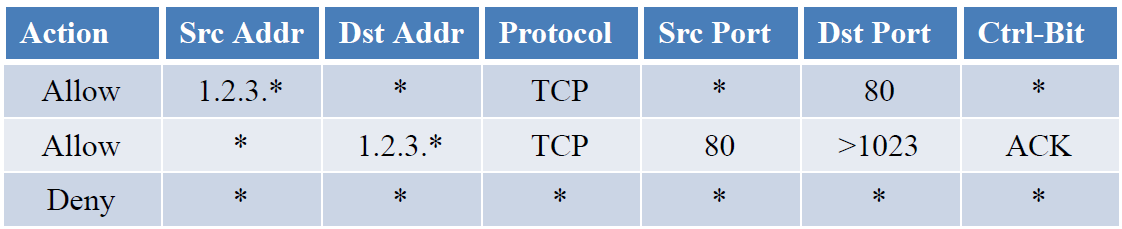
\includegraphics[width=0.7\columnwidth]{stateless-filter}
\end{center}
\subsubsection{Stateful Packet Filters}
\begin{itemize}
	\item Maintains a state table of all active connections
	\item Filters packets based on connection states
\end{itemize}
\subsubsection{Proxy-based or Application Firewalls}
\begin{itemize}
	\item Understands application logic
	\item Acts as a relay of application-level traffic
\end{itemize}
\subsubsection{Netfilter: Linux Firewall}
\begin{minipage}{0.3\columnwidth}
	\begin{center}
		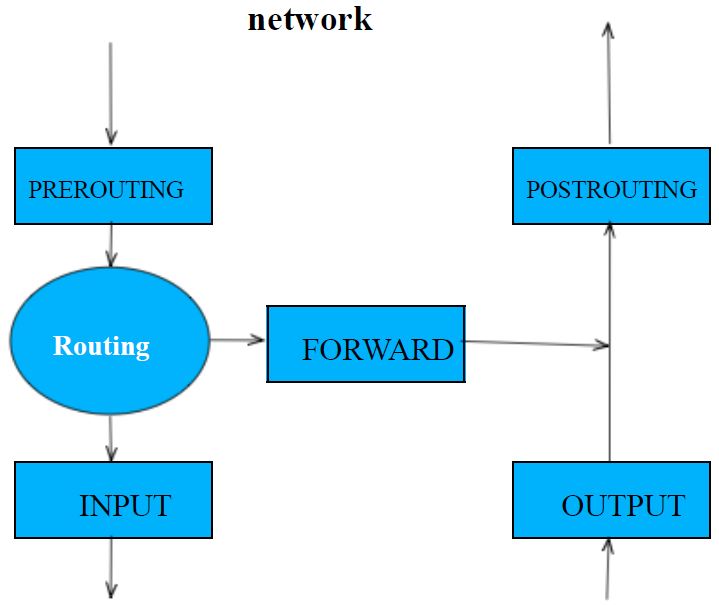
\includegraphics[width=1\columnwidth]{netfilter}
	\end{center}
\end{minipage}
\begin{minipage}{0.5\columnwidth}
Five hooks to decide the fate of a packet
\begin{itemize}
	\item Prerouting
	\item Postrouting
	\item Forward
	\item Input
	\item Output
\end{itemize}
\end{minipage}
\subsubsection{Threat Model}
\begin{itemize}
	\item Goal:
	\begin{itemize}
		\item Stop attacker’s packet from reaching the end application
	\end{itemize}
	\item Adversary Capability
	\begin{itemize}
		\item Adversary can send malicious network packets
		\item Adversary is outside the network perimeter
	\end{itemize}
	\item Assumptions
	\begin{itemize}
		\item network perimeter is correctly defined
		\item firewall is uncompromised (not buggy)
		\item firewall sees the same data as end application (need to account for differences in assembly of packets)
		\item Defender’s policy can tell bad from good traffic by inspecting packet content
	\end{itemize}
\end{itemize}

Assuming assumptions are true:
\begin{itemize}
	\item possible to prevent slammer worm by blocking port 1434
	\item possible to break signature filter by splitting signature across packets
	\item possible to prevent ICMP attacks by blocking broadcast channel
	\item impossible to prevent DDoS attack if it is sent by infected host within network
	\item threats coming from legitimate ports requires additional checks of content and signatures
\end{itemize}
\subsubsection{Weaknesses of Threat Model}
\begin{itemize}
	\item Defender needs to know all possible attacks and how to block them for firewalls to be effective - easy for attackers to evade those attack patterns
	\item Enforcement is very complex
	\item Continuous arms race, e.g. evolving signatures
	\item Easy to violate assumptions
	\begin{itemize}
		\item Physically Compromise the firewall
		\item Difficult to ascertain which service is targeted from inspecting network flows only
		\item Firewall network code may differ from host OS / app code
		\item Many attack (raw byte) patterns for the same exploit!
	\end{itemize}
	\item Thwarted completely by encrypted traffic (e.g. HTTPS)
	\item “Bring your own device” problem: Carrying data on a smartphone from outside the network
\end{itemize}
\section{Secure Channel}
A Secure Channel is a data communication protocol established between 2 programs which preserves data in terms of
\begin{itemize}
	\item \textcolor{red}{C}onfidentiality
	\item \textcolor{red}{I}ntegrity
	\item \textcolor{red}{A}uthentication/Authenticity (person we are talking to is who they say they are)
\end{itemize}
* Availability is not a goal!! DDoS attacks permitted by threat model
\subsection{Basic Cryptographic Primitives}
\begin{itemize}
	\item Encryption \textbf{only provides Confidentiality} promise and does not guarantee Integrity and Authenticity
	\item MAC \& Digital Signature \textbf{provides both integrity and authenticity} guarantees but does not guarantee confidentiality
	\item Example of Secure Channels
	\begin{itemize}
		\item HTTPS, Encrypted File System, SSH/VPN
	\end{itemize}
\end{itemize}
\subsection{Symmetric Key Encryption}
Assume that Alice is communicating with Bob and a malicious attacker A is in between them that is capable of eavesdropping and modifying packets. To prevent attacker, we have 2 options:
\begin{itemize}
	\item Assume A has poorer network than Alice/Bob and receive less data than Alice/Bob
	\item Assume Alice and Bob have some pre-shared secret key
\end{itemize}
\subsubsection{How it works}
\begin{enumerate}
	\item Alice and Bob first preshare a secret key $K$ which is randomly generated
	\item Encryption: $M\times K \rightarrow C$
	\item Decryption: $C\times K \rightarrow M$
\end{enumerate}
Must ensure that it follows the correctness property: $\forall m,k, Dec\left(Enc(m,k)\right)=m$
\subsubsection{Adversary's Knowledge}
\begin{itemize}
	\item Algorithms Setup, Enc, Dec are public, but internal coin flips are private (makes generation of key probabilistic)
	\item Adversary knows any distribution over M from background knowledge but defender does not
\end{itemize}
\subsubsection{Chosen Plaintext Attack}
\begin{itemize}
	\item Attacker has access to encryption oracle
	\item Attacker can repeatedly try sending plaintext over to oracle and check whether the encrypted text matches
\end{itemize}
\subsubsection{Security}
Want to achieve perfect secrecy: $Pr[Guess=m|c] = Pr[Guess = m]$, i.e. even if attacker know ciphertext, it is just as good as guessing without any prior knowledge
\subsubsection{Caesar Cipher}
\begin{itemize}
	\item Idea is that the key is the number of times to rotate the characters by
	\item C = (P + X) mod 26 where X is the number of rotations
	\item Easily broken once we know the (Setup, Enc, Dec) operations
	\item Deterministic functions, easily subject to frequency analysis
\end{itemize}
\subsubsection{One time pad}
\begin{itemize}
	\item Enc: $c:=m\oplus k$, k is the randomly chosen secret key
	\item Dec: $m=c\oplus k$
	\item k changes for each plaintext message
	\item Achieves correctness and perfect secrecy
	\item $|K|\geq |M|$, requires a huge key space $\rightarrow$ if can securely transfer $K$ then can also securely transfer $M$
	\item Relies on bijection of M $\rightarrow$ C, if not there will be some c then shows up more frequently and will be susceptible to dictionary attacks
	\item \# of functions that can be defined from $n$-bits to $m$-bits $=2^{m\cdot2^n}$
\end{itemize}
\subsection{Integrity}
In a normal communication setup, Bob would not be able to distinguish data sent by Alice vs Attacker. Checksums are useless too since they are keyless and is only used for error correction
\subsubsection{Message Authentication Codes (MAC)}
Provides sender Authenticity and integrity of messages sent.

\underline{How it works}
\begin{enumerate}
	\item Sender generates a tag: $S(k, m)$ which basically "signs" the message with a secret key that is pre-shared
	\item Sender sends message $m$ with the tag
	\item Receiver then verifies $V(k,m,\text{tag})$ which detects whether any changes has been made to the message and at the same time verifies that it is the correct key (and hence is the authentic sender)
\end{enumerate}
\subsubsection{Formal Security Goal for MAC}
\begin{itemize}
	\item Want to prevent existential forgery under Chosen Message Attack (CMA)
	\begin{itemize}
		\item Given $m$, $Pr[V(k,m,t)\rightarrow yes] \leq negl$, where $t$ is a tag guessed by Attacker
	\end{itemize}
\end{itemize}
\subsubsection{Perfectly Secure MAC}
$$(a\cdot m+b)modp$$
where $m,p$ is known publicly and $(a,b)$ is the secret key that is chosen randomly
\begin{itemize}
	\item Works on universal hash family
	\item $Pr[S_{a,b}(m)=t\land S_{a,b}(m')=t']=\frac{1}{|T|^2}$
	\item Key space $|K|$ for perfectly secure MAC is $2n$ for $n$ bit MAC to make it such that attacker has negligible chance of success
\end{itemize}
\subsection{Takeaways}
\begin{itemize}
	\item Symmetric Key Constructions are feasible but having perfect secrecy and perfect MACs take up way too much space and are impractical
\end{itemize}
\subsection{Relaxed Assumption of Attacker}
\begin{itemize}
	\item Assumes that adversary has limited computation power
	\item Adversary can execute polynomial \# of steps
	\item Has randomized and non-deterministic execution
	\item Bounds queries in CPA/CMA to polynomial in |K| i.e. if key bits is 128, adversary can't compute all $2^{128}$ computation
\end{itemize}
\subsection{Public Key Cryptography}
Instead of having a pre-shared secret key, both Alice and Bob now have a pair of public and private key
\begin{itemize}
	\item e.g. Alice wants to send Bob a message, Alive will encrypt the message using Bob's public key and Bob will decrypt using his own private key
	\item Can also be used to do signature by signing message with private key and receiver can verify it using the public key
	\item Works under the assumptions:
	\begin{itemize}
		\item Difficulty of Factoring product of large primes - circumvented by quantum computing
		\item Discrete Logarithm in Groups is computationally difficult
		\item Problems in Lattices - withstand quantum computing adversary
	\end{itemize}
\end{itemize}
\subsubsection{Key Exchange Protocol}
\begin{itemize}
	\item Used to establish fresh shared secrets per session
	\item Session keys is a means to maintain (Perfect) forward secrecy $\rightarrow$ protect encrypted information even if long term key is compromised
	\item Based on computational hardness assumption of Discrete Log (DLOG)
	\begin{itemize}
		\item For an appropriately chosen group $G$ (e.g. Integer mod prime), where $g$ is the generator. Given $A\in G$, difficult to find any $a\in G$ such that $g^a=A$ (for any "classical" computer)
		\item Can be interpreted as how many times do we run the generator to get A
	\end{itemize}
\end{itemize}
\subsubsection{Diffie Hellman}
\begin{center}
	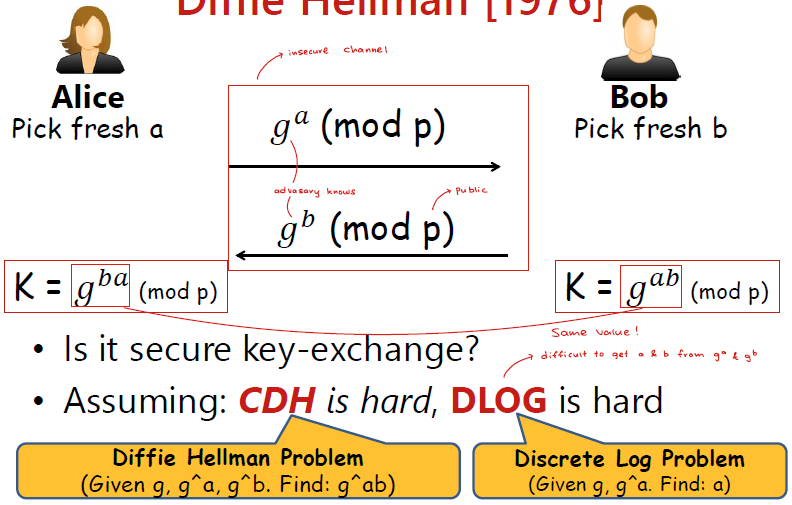
\includegraphics[width=0.7\columnwidth]{diffie-hellman}
\end{center}
\begin{itemize}
	\item Eve sees $g^a,g^b$
	\item Under Computational Diffie-Hellman (CDH), it is computationally hard to compute $g^{ab}$
	\item Under Decisional Diffie-Hellman (DDH), $g^{ab}$ looks like a random element from $G$
	\item DH Key Exchange is secure against Eve
\end{itemize}
\begin{center}
	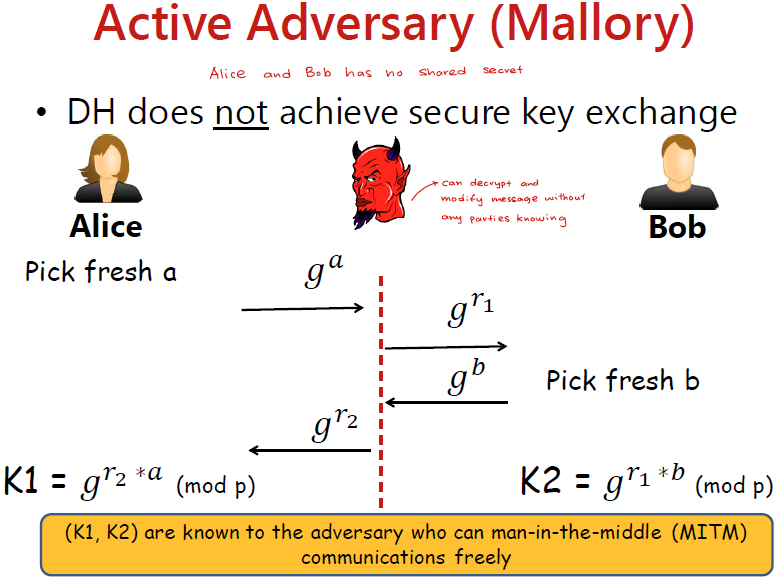
\includegraphics[width=0.7\columnwidth]{diffie-hellman-mallory}
\end{center}
\begin{enumerate}
	\item MITM can intercept $g^a$ sent by Alice and send $g^{r_1}$ to Bob 
	\item Bob will then send back $g^b$ which is also intercepted by MITM and sends Alice back $g^{r_2}$
	\item Alice now has $g^{r_2*a}$ (mod p) and Bob has $g^{r_1*b}$ (mod p) and MITM has both the $r_1$ and $r_2$ 
\end{enumerate}
\subsubsection{Authenticated Key Exchange}
\begin{itemize}
	\item Authentication key exchange protocol guarantees
	\begin{itemize}
		\item Entity Authentication: Entities are who they claim to be
		\item Good Key: Only the intended parties derive shared new secret
	\end{itemize}
\end{itemize}
\underline{Station-to-station (STS) Protocol}\\
\begin{minipage}{0.5\columnwidth}
	\begin{center}
		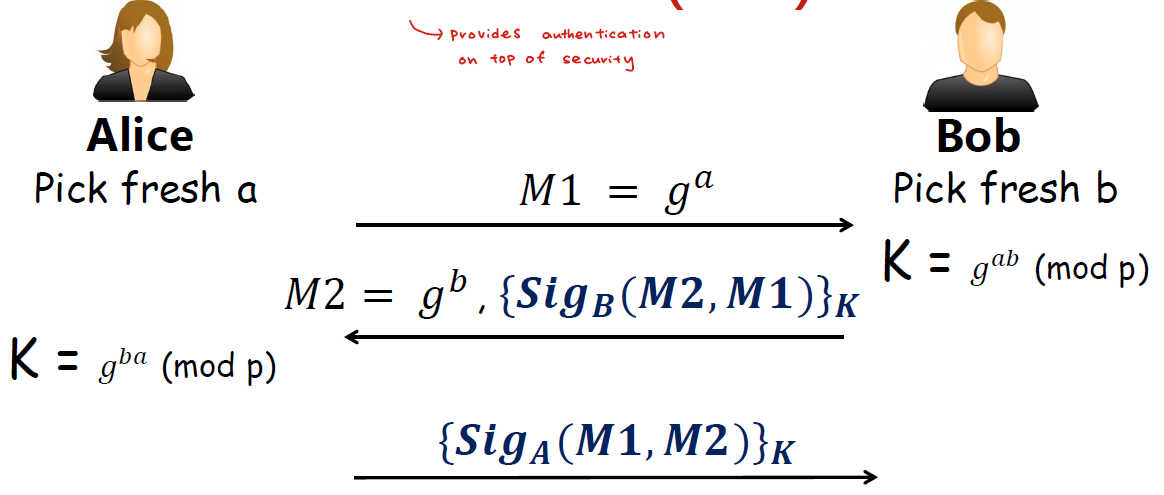
\includegraphics[width=1\columnwidth]{station-to-station}
	\end{center}
\end{minipage}
\begin{minipage}{0.6\columnwidth}
	\begin{itemize}
		\item STS provides both authentication and security promises 
		\item Secure against both Eve and Mallory
	\end{itemize}
\end{minipage}
\vfill\null
\subsection{HTTPS}
\begin{itemize}
	\item HTTP + Secure Socket Layer (SSL) = HTTPS
	\item Modern SSL is known as TLS and is continually revised to prevent more threats
\end{itemize}
\subsubsection{High Level Implementation of SSL/TLS}
\begin{center}
	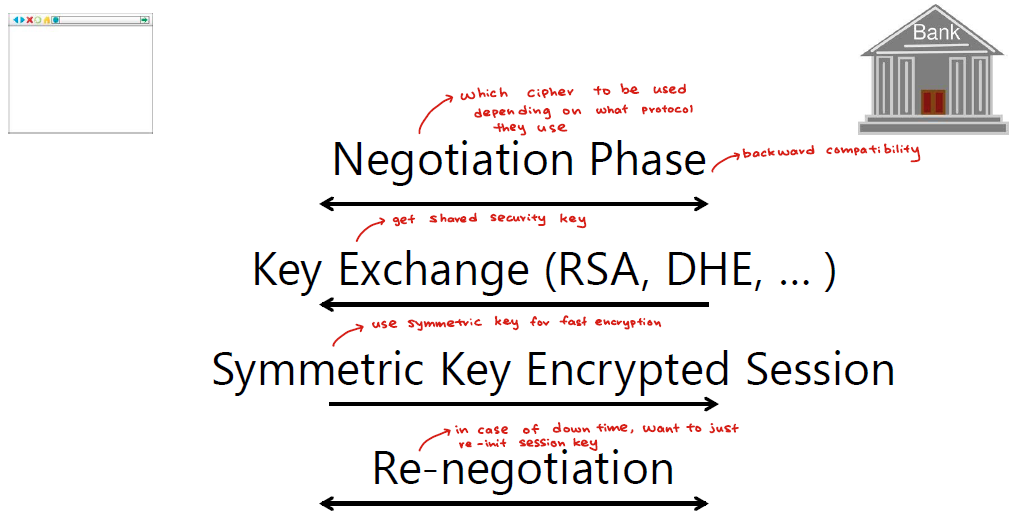
\includegraphics[width=0.8\columnwidth]{tls}
\end{center}
\begin{itemize}
	\item Negotiation phase: what cipher is used that is compatible to both server and client, provides backward compatibility
	\item Key Exchange using RSA, DHE etc., session key is generated here
	\item Symmetric Key is used to encrypt the entire session $\rightarrow$ Symmetric key used instead of public-private key since it provides much faster encryption, private-public key requires a lot of bits to be safe
\end{itemize}
\subsubsection{Certificates}
\begin{itemize}
	\item Guarantees Integrity and Authenticity
	\item Similar to Digital Signatures but for Web
	\item Certificates are signed by Certificate Authorities (CA)
	\begin{itemize}
		\item Root CA's public keys are hard coded into OS
		\item Chain of Trust stops at root CA
	\end{itemize}
	\item Root CAs can designate intermediate CAs (restricted to signing own subdomain)
	\item Based on trust system where we completely trust that root CAs are not malicious
\end{itemize}
\subsubsection{HTTPS Implementation}
\begin{center}
	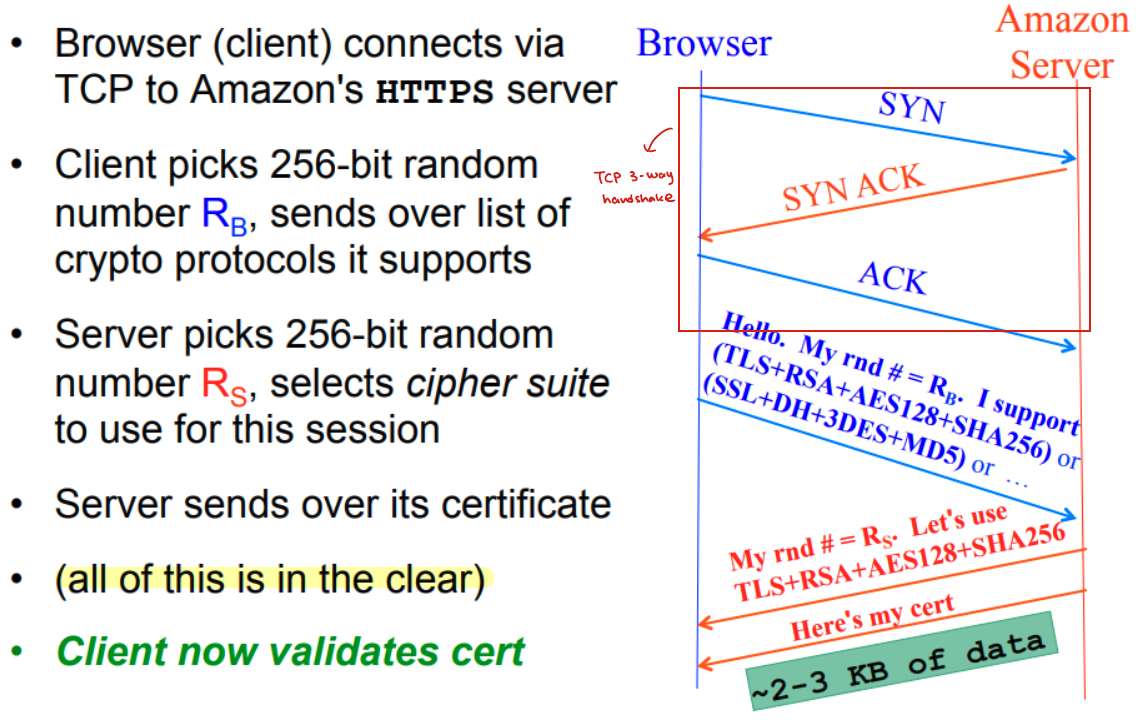
\includegraphics[width=0.8\columnwidth]{tls-implementation}
\end{center}

\underline{RSA Implementation}
\begin{itemize}
	\item Does not have forward secrecy guarantee, once attacker gets PS, whole encrypted channel is exposed
\end{itemize}
\begin{center}
	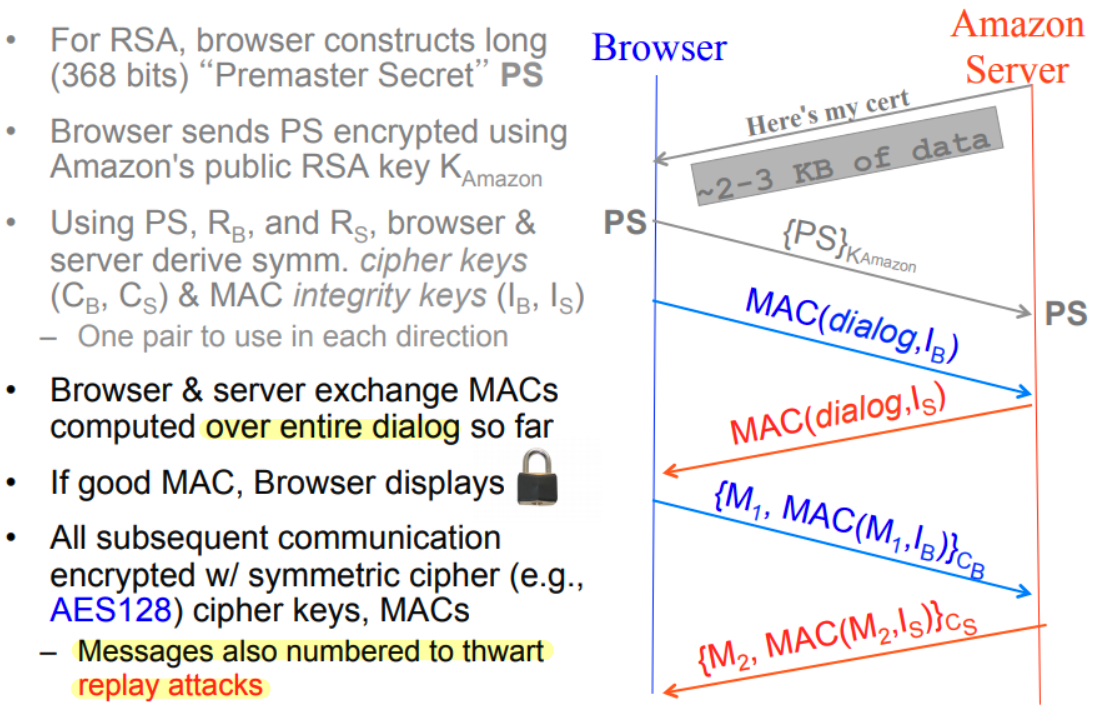
\includegraphics[width=0.8\columnwidth]{rsa}
\end{center}
\underline{Diffie-Hellman Implementation}
\begin{center}
	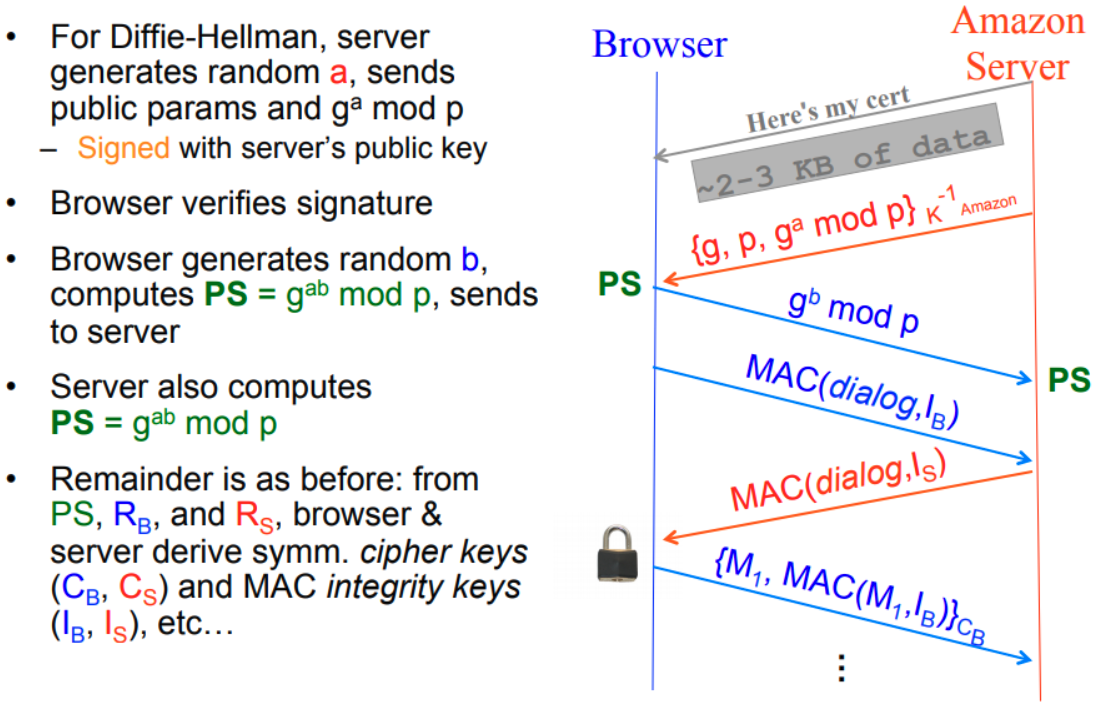
\includegraphics[width=0.8\columnwidth]{dhe-tls}
\end{center}
\subsubsection{Assumption of Threat Model}
\begin{itemize}
	\item User is using a secure channel
	\item Crypto primitives are secure (uses RSA, HMAC etc.)
	\item TLS protocol design is secure
	\item TLS protocol implementation is secure
	\item Certificate issuers are uncompromised
	\item Users check browser UI correctly
	\item Alice \& Bob’s secrets are secure
	\item Entities are authenticated correctly
\end{itemize}
\subsubsection{Capabilities of HTTPS}
\begin{itemize}
	\item Assuming that we reach https://gmail.com and it shows no cert errors, we can safely assume that it is safe from ALL network attacks
	\begin{itemize}
		\item Safe from DNS cache poisoning (will not show padlock since they don't have server's certificate)
		\item Safe from BGP route hijacking (again certificates won't match)
		\item Safe from TCP/IP attacks (data streams are encrypted and attacker can't see seq \#)
	\end{itemize}
	\item Everything of an URL except IPs and ports are encrypted when using HTTPS
\end{itemize}
\subsubsection{Downfalls of HTTPS}
Typical ways attackers can "win" by going outside of the threat model:
\begin{itemize}
	\item Attack assumptions
	\item Violate other security properties that are not captured by threat model e.g. attack availability instead
\end{itemize}
\underline{HTTP Downgrade Attack}
\begin{itemize}
	\item Mallory is on the network and downgrades traffic from HTTPS to HTTP
	\item Possible to downgrade other sub-resources on page to HTTP (e.g. Script tags, img src, iFrames etc.)
	\item Assume that as long as HTTP then IT IS NOT SAFE
	\item Can be prevented by using HTTP Strict Transport Security (HSTS) which is a header that states that your website only serves HTTPS sites
\end{itemize}
\underline{Insecure Cookies}
\begin{itemize}
	\item Possible to use an img src to a HTTP site that will leak cookies to HTTP traffic
	\item Prevented by setting "secure" flag for cookies which tells browser not to send cookies over HTTP
	\item Cookies are only sent securely through HTTPS and 'Secure' Keyword but can be read by JS via DOM API (if JS is injected then everything will fail)
	\item Cookies could be overriden by HTTP request (\texttt{Set-cookie: SID=bad;secure}) 
	\item Cookies could be overriden /deleted by JS: evil.example.com can set cookies for example.com
\end{itemize}
\underline{UI Confusion}
\begin{itemize}
	\item bankofthewest.com VS bankofthevvest.com
	\item null byte certificate e.g. gmail.com\textbackslash0.evil.com will be read as gmail.com from browser perspective
	\item p\&\#1072;ypal.com shows up as accented 'a' in browser which is almost indistinguishable from normal 'a'
	\item In general note that everything below the address bar is unreliable!
\end{itemize}
\underline{Clickjacking}\newline
\begin{minipage}{0.6\columnwidth}
	\begin{center}
		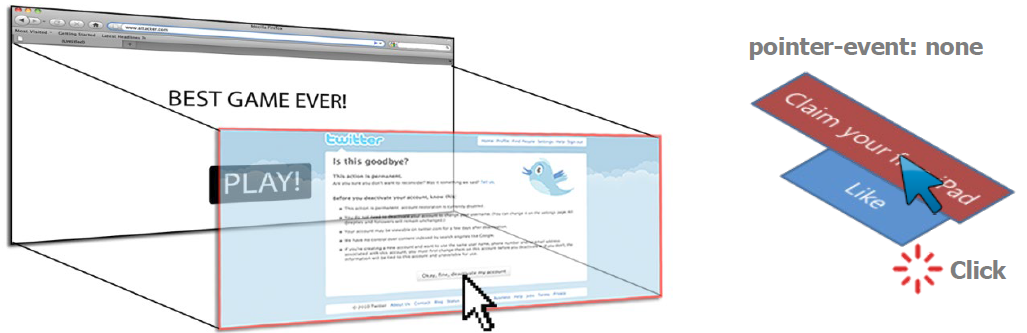
\includegraphics[width=1\columnwidth]{clickjacking}
	\end{center}
\end{minipage}
\begin{minipage}{0.4\columnwidth}
	\begin{itemize}
		\item Possible to embed iframes into pages that can host any site
		\item Frames of iframe can overlap and can even be made transparent / makes clicks fall through it by using CSS
	\end{itemize}
\end{minipage}
\underline{Compromised Cert / CA}
\begin{itemize}
	\item How to detect if being served bad cert
	\begin{itemize}
		\item Certificate pinning (used in SSH, "trust on first use", cache certificates after first visit)
		\item Certificate Revocation (allows CA to remove certs that are found malicious)
		\item Certificate Transparency (allows people to check CA's cert and store it in a Public Cert. Log)
	\end{itemize}
\end{itemize}
\underline{Side Channel Attacks}
\begin{itemize}
	\item Size of data, Data access patterns (fixed using deterministic address pattern or randomization), power channel, sound, electromagnetic radiation
	\item Timing Channel
	\begin{itemize}
		\item exploit variations in execution time of a program or system based on different inputs or conditions
		\item solved by ensuring that computation time does not differ much between branches
	\end{itemize}
\end{itemize}
\underline{Broken Crypto Primitive}
\begin{itemize}
	\item Using MD5 which is prone to collisions
	\item Using encrypt-and-MAC instead of MAC-then-encrypt (SSL, could be insecure by using padding oracle) or encrypt-then-MAC (IPSec, provably secure)
\end{itemize}
\section{Extra Content}
\subsection{DNSSEC}
\begin{itemize}
	\item DNS is unsafe since we do not know whether the reply is sent from the authentic DNS server and we also do not know whether the final A record is tampered
	\item DNSSEC prevents this by adding on signatures to each DNS reply
	\item Each DNS server stores 2 or more key pairs and hashes of its own child zone keys
\end{itemize}
\begin{center}
	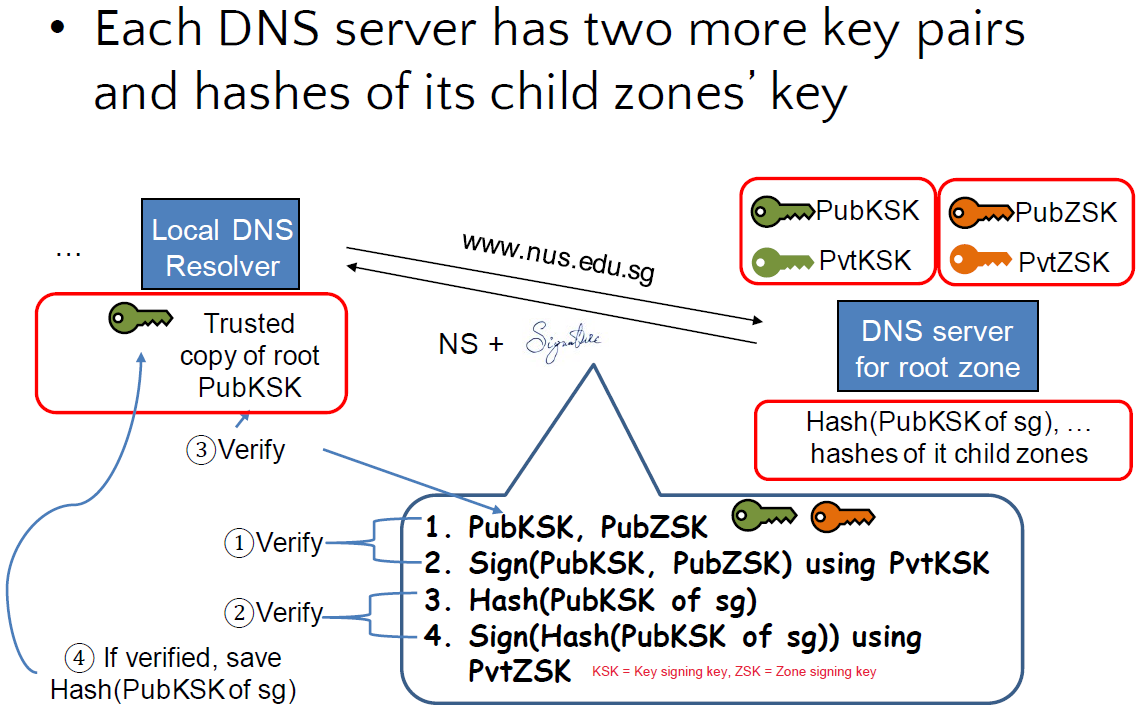
\includegraphics[width=0.7\columnwidth]{dnssec}
\end{center}
\begin{itemize}
	\item Purpose: Ensures that replies from DNS servers are authentic and that the final A records are not tampered with
	\item Attacks prevented: MITM and DNS cache poisoning and QID prediction attack
	\item Assumptions: DNS servers are not compromised and that the root DNS KSK must be trusted
\end{itemize}
\subsection{DANE}
\begin{itemize}
	\item Resolves issue of TLS having heavy reliance on the chain of trust $\rightarrow$ possible that CAs wrongly issues certificates
	\item Can be used by HTTPS and SMTP
\end{itemize}
\begin{center}
	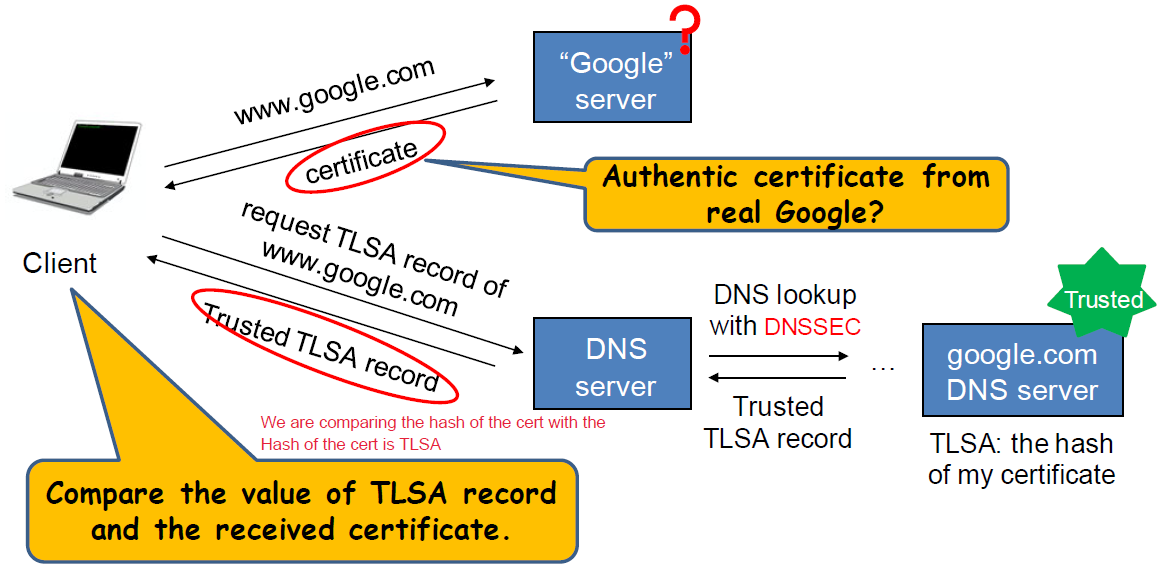
\includegraphics[width=0.7\columnwidth]{dane}
\end{center}
\begin{itemize}
	\item Uses DNSSEC to check authenticity of certificates
	\item Prevents impersonation even if CAs wrongly issues certificates
\end{itemize}
\subsection{SPF}
\begin{itemize}
	\item Specifies the servers and domains that are authorized to send email on behalf of your organization
	\item SPF records are basically DNS TXT records that acts as a whitelist for authorized servers
	\item Receiver can just verify that the sender is indeed authorized to send by checking the IP address of SPF
	\item Prevents email spoofing
	\item Attacker can only bypass SPF by gaining access to IP address of email server which is hard in practice
\end{itemize}
\subsection{DKIM}
\begin{itemize}
	\item Adds a digital signature to every outgoing message, which lets receiving servers verify the message actually came from your organization
	\item Domain owner add a DKIM key in DKIM TXT record
	\item Sender is expected to sign the email
	\item Receiver will add Authentication-Resultsheader (DKIM=pass/OKindicates verified mail)
	\item Another way to prevent email spoofing attacks by adding a layer of authenticity to the email messages through signatures
	\item Assumes that Key management and TTLs are in place
\end{itemize}
\subsection{DMARC}
\begin{itemize}
	\item Additional notification protocol for messages that do not pass DKIM or SPF.
	\item DMARC records will store an email address which will receives reports if any of the above 2 protocols fails
\end{itemize}
\subsection{PGP}
\begin{itemize}
	\item Web of trust —decentralized, accumulate and distribute public keys
\end{itemize}
\begin{center}
	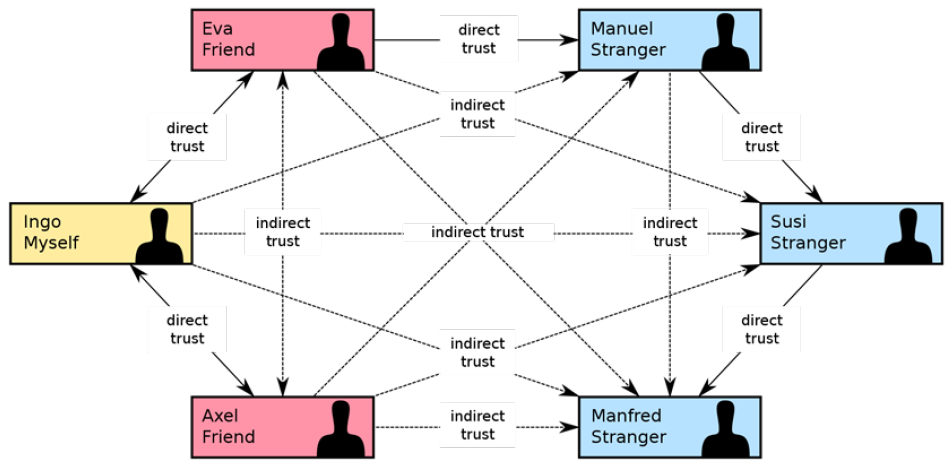
\includegraphics[width=0.7\columnwidth]{pgp}
\end{center}
\end{multicols*}
\end{document}
